\chapter{\"Ubersicht}
\section{Motivation}
Dieses Dokument wurde erstellt um eine einheitlich Enwicklungsumgebung zu schaffen und die Vorgaben der Entwickler zu erhalten.

Vorteile bei der Einhaltung der Richtlinien sind eine raschere Einarbeitung ins System sowie der Erweiterung von Programmteilen.

\newpage

\section{Entwicklungsumgebung}

Die Standard Entwicklungsumgebung am Technikum-Wien ist Eclipse PDT (PHP Development Tools Project) oder Netbeans.

\href{http://www.eclipse.org/pdt/}{http://www.eclipse.org/pdt/} (Stand 16.11.2012) \newline
\href{http://netbeans.org/features/php/}{http://netbeans.org/features/php/} (Stand 16.11.2012)

\newpage
\section{Ordnerhierarchie}

Ordnerhierarchie des FH-Complete Systems

\begin{figure}
	\centering
	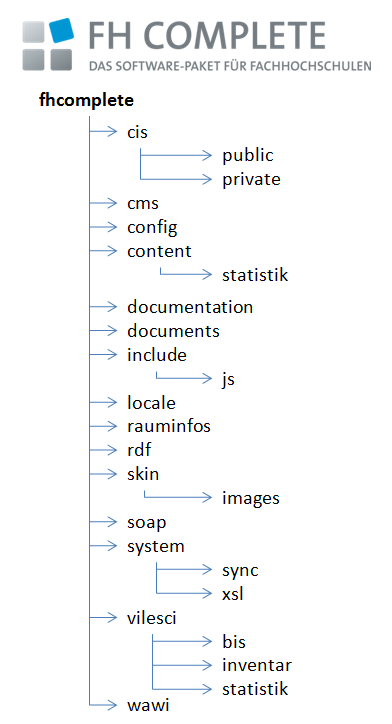
\includegraphics[width=0.65\textwidth]{Kodierrichtlinien_Ordnerhierarchie.png}
	\caption{Ordnerhierarchie von FH-Complete}
	\label{Ordnerhierarchie}
\end{figure}

\newpage
{\bf/cis:} Dateien speziell f\"ur das CIS System
\begin{itemize}
	\item{{\bf/public:} \"offentlich sichtbar}
	\item{{\bf/private:} Student/User muss eingeloggt sein um Content zu sehen (.htaccess)}
\end{itemize}

{\bf/cms:} Dateien f\"ur das CIS Content Management System und Document Management System

{\bf/config:} In diesem Ordner sind alle Konfigurationsdateien gespeichert (CIS, WAWI, VILESCI, Global) 

{\bf/content:} XUL Dateien FAS / TEMPUS / PLANNER
\begin{itemize}
	\item{{\bf/statistik:} Statistiken}
\end{itemize}

{\bf/dokumentation:} Dokumentation und Benutzerhandb\"ucher aller Systeme

{\bf/documents:}

{\bf/include:} Klassen und FH Spezifisches
\begin{itemize}
	\item{{\bf/js:} JavaScript Bibliotheken (JQuery)}
	\item{{\bf/tw:} Men\"ueintr\"age f\"ur Technikum Wien}
\end{itemize}
{\bf/locale:} Sprachdateien f\"ur FAS oder Sprachenmodul

{\bf/rauminfos:} Rauminfos aller R\"aume in HTML Files

{\bf/rdf:} RDF Files, zur PDF Erstellung ben\"otigt (Zeugnis, Bestellschein,..) 

{\bf/skin:} CSS Datein 
\begin{itemize}
	\item{{\bf/images:} Grafiken und Bilder f\"ur die Systeme}
\end{itemize}

{\bf/soap:} Alle Dateien f\"ur Webservices

{\bf/system:} Verwaltungsskripte 
\begin{itemize}
	\item{{\bf/sync:}}
	\item{{\bf/xsl:}}
\end{itemize}

{\bf/vilesci:} Dateien speziell f\"ur VILESCI
\begin{itemize}
	\item{{\bf/bis:} Bismeldungsrelevanten Daten}
	\item{{\bf/inventar:} Inventarprogramm}
	\item{{\bf/statistik:} Statistiken}
\end{itemize}

{\bf/wawi:} Files f\"ur WaWi

\section{Server\"ubersicht}

{\bf Sirene:} CIS, FHComplete, Moodle, Opus \newline
{\bf Fhctemp:} FAS, Tempus, Vilesci \newline
{\bf Theseus:} Datenbankserver (Postgres, MySQL) \newline
{\bf Calva:} Entwicklungsserver \newline